%!TEX root = ../../thesis.tex

The \ac{LHC} is the world's largest and most energetic particle accelerator. It is 
installed in a \unit{27}{\kilo\metre} tunnel at a mean depth of \unit{100}{\metre} beneath 
the French--Swiss border, which was previously occupied by the \ac{LEP}. It accelerates 
beams of protons (or lead ions) to high energy and then collides them within the
ATLAS, CMS, LHCb and ALICE detectors. Although the design \ac{CM} collision energy is 
\unit{14}{\TeV}, it operated at \unit{7}{\TeV} and \unit{8}{\TeV} during run I, as 
described in \Section~\ref{sec:dataset}.

The \ac{LHC} proton beams have humble beginnings as hydrogen molecules in a standard gas 
bottle, before being stripped of their electrons and entering the \ac{LHC} accelerator 
complex shown in \Figure~\ref{fig:lhc}. The \ac{LHC} accelerator features 16 
radio-frequency cavities to provide acceleration and restore energy losses, 1232 
dipole magnets to bend the beam into a nearly circular path, 392 quadrupole magnets to 
focus the beam, and many other magnetic components. Most of these magnets rely on 
unprecedented superconducting twin-bore magnet technology operating at cryogenic 
temperatures.

\begin{figure}
	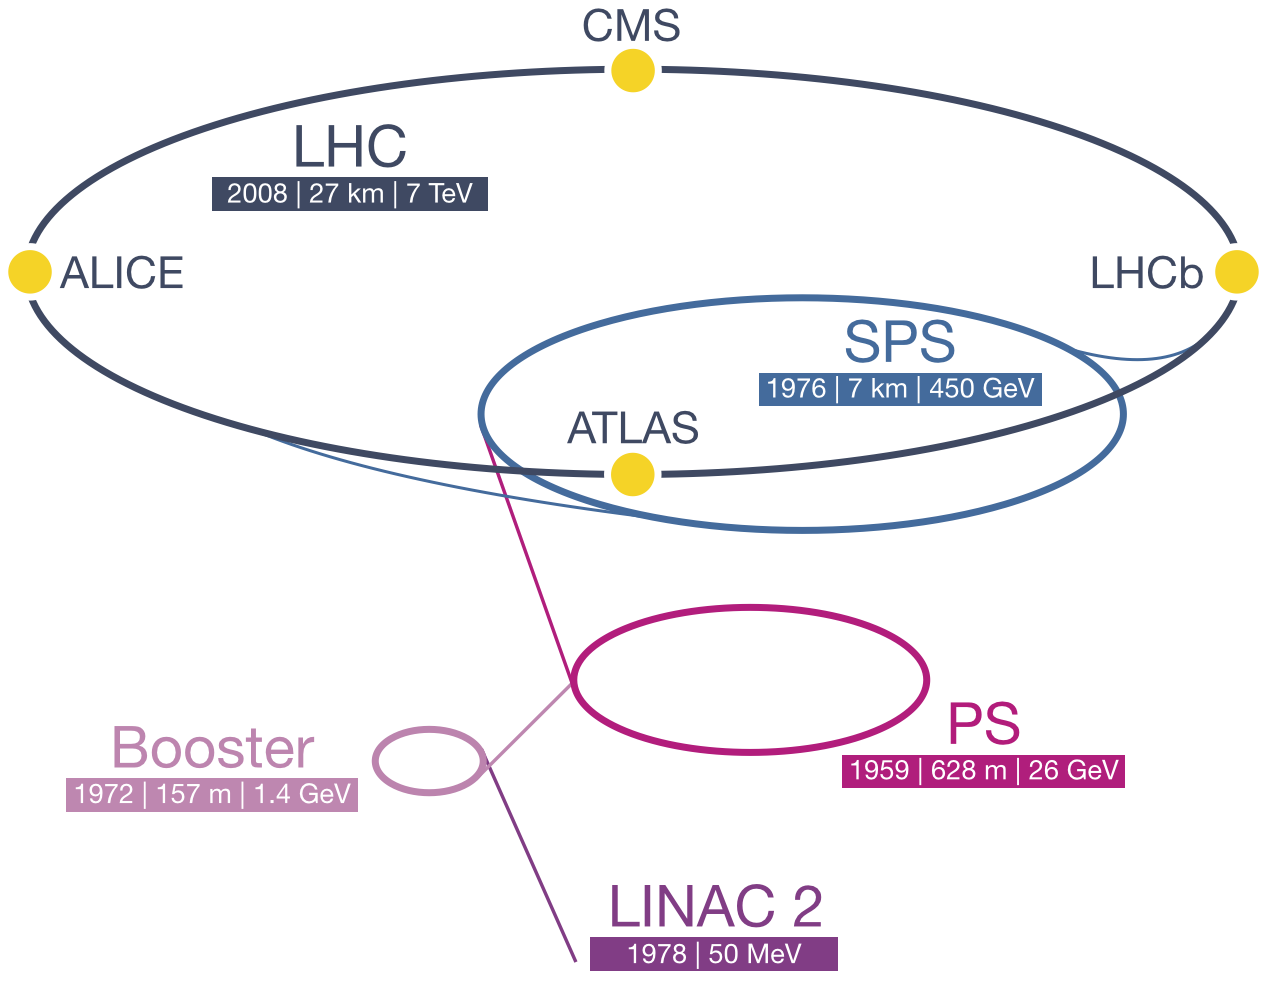
\includegraphics[width=\largefigwidth]{tex/experiment/lhc}
	\caption{The \ac{LHC} accelerator complex at CERN. The successively higher energy 
	accelerators are: Linear Accelerator 2 (LINAC 2), Proton Synchrotron Booster, Proton 
	Synchrotron (PS), Super Proton Synchrotron (SPS), and finally the \acf{LHC}. The four 
	main \ac{LHC} detectors are also shown.}
	\label{fig:lhc}
\end{figure}

For experiments to be sensitive to rare processes with small cross sections, such as Higgs 
boson production, the detectors must record a large integrated luminosity. This is seen by 
considering the expected number of events produced for process $i$
\begin{equation}
	N_i = \sigma_i \! \int \! L \, \diff t
	\label{eq:event_rate}
\end{equation}
where $\sigma_i$ is the cross section and $L$ is the instantaneous luminosity, a figure of 
merit for a collider. The instantaneous luminosity can be increased by optimising the
parameters of
\begin{equation}
	L = \frac{N_b^2 n_b f_{\text{rev}}}{4\pi \varSigma_x \varSigma_y} F
	\label{eq:lumi_beam}
\end{equation}
where $N_b$ is the number or particles per bunch, $n_b$ is the number of bunches per beam, 
$f_{\text{rev}}$ is the revolution frequency, $\varSigma_x$ and $\varSigma_y$ are the $x$ 
and $y$ components of the beam size, and $F$ is a reduction factor due to the crossing 
angle at the interaction point. The \ac{LHC} is designed to hold 2808 proton bunches, 
corresponding to \unit{25}{\nano\second} bunch spacing, each containing $1.15\times10^{11}$
protons. The other design parameters are \unit{$\varSigma_{x,y} = 16.7$}{\micro\metre} 
and \unit{$f_{\text{rev}} = 11.25$}{\kHz}, giving a design luminosity of 
\unit{$L \approx 10^{34}$}{\lumiunits} \cite{LHC}.

A trade-off for higher luminosity is a larger number of additional proton-proton 
interactions, known as pile-up. Although a rare interesting event will trigger the 
detector readout, these common uninteresting events will simultaneously be recorded, 
obscuring the interesting physics and degrading detector performance. Increasing $N_b$ 
gives more interactions within the same bunch crossing, known as in-time pile-up. For 
large $n_b$, the bunch spacing can be shorter than the detector latency, and interactions 
from other bunch crossings can affect the measurement - this is known as out-of-time 
pile-up. Reducing $\varSigma_{x,y}$ will increase both types of pile-up.
